\section{指针与数组的复合类型}
在前面的几节中我们可以看到,指针和数组之间有着千丝万缕的联系,它们虽然类型不同,但都与内存地址密不可分。数组类型还可以转换成指针类型,这种情况在参数传递中普遍存在。\par
本节我们来研究一些更复杂的结构:二维数组、指针数组、指向数组的指针和指向指针的指针(二阶指针)。它们的分析方法和我们分析一维数组和一级指针的方式大体相同,不过在这里我们要更多地关注类型信息。\par
\subsection*{二维数组}
定义二维数组的基本语法如下:
\begin{lstlisting}
int darr1[2][3] = {{1,2,3},{4,5,6}}; //正常格式,注意是外层2个,内层3个,勿搞反
int darr2[3][3] {{7,8},{10}}; //每个花括号内可分别省略内容,省略的部分初始化为0
int darr3[][4] {{1,2,3,4},{5,6},{}}; //只能省略第一维长度,不能省略第二维长度
\end{lstlisting}
初学者很容易在二维数组的下标问题上犯糊涂。比如,在定义 \lstinline@darr1@ 的时候,究竟是要写成\linebreak\lstinline@{{1,2,3},{4,5,6}}@ 还是要写成 \lstinline@{{1,2},{3,4},{5,6}}@?还有,\lstinline@int[2][3]@ 和 \lstinline@int[3][2]@ 到底有什么区别?为什么在定义 \lstinline@darr3@ 的时候只能省略第一维的长度而不能省略第二维的长度?\par
要解决这些问题,我们就要去探寻二维数组的本质。\par
\subsubsection*{二维数组是什么?}
我们已经对一维数组十分熟悉了。在我们已有的理解中,一维数组是内存中连续的一串数据,每个元素的类型都是基本数据类型。比如说 \lstinline@int arr[3]@ ,它就是一个一维数组,类型为 \lstinline@int[3]@;而它的某个元素,比如 \lstinline@arr[0]@,就是一个数据,类型为 \lstinline@int@。我们可以把它叫做``由数据构成的数组''。\par
那么我能否定义一个``由数组构成的数组''呢?假设我们想定义一个由4个 \lstinline@arr[3]@ 数组构成的数组,那么我们岂不是应该定义成 \lstinline@int (darr[3])[4]@?\par
这就错了——其实这也是初学者常常会出现的理解误区。为了便于我们清晰地理解指针/数组复合类型的定义,请读者记住一条重要原则:\textbf{``定义的语法''要与``使用的语法''保持一致。}\par
以刚才说到的二维数组为例。我们希望定义一个长度为4的二维数组 \lstinline@darr@,这个数组的每个元素都是一个长度为3的数组。那么在我们使用的时候,\lstinline@darr[0]@ 就是一个长度为3的数组吧!同样的,\lstinline@darr[1]@, \lstinline@darr[2]@ 和 \lstinline@darr[3]@ 都是一个长度为 \lstinline@3@ 的数组。\par
那么,如果我们还要再读取更内层的信息(这次就是数据了,或者说是二维数组的元素),我们就需要把 \lstinline@darr[i]@ 当作一个整体,再用一次下标运算符,也就是 \lstinline@(darr[i])[0]@, \lstinline@(darr[i])[1]@ 和 \lstinline@darr[i][2]@(可以省略括号,不影响结果)。\par
那么回顾一下 \lstinline@darr[i][j]@ 这个语法,其中 \lstinline@i@ 的合理范围是 \lstinline@0@\~{}\lstinline@3@,而 \lstinline@j@ 的合理范围是 \lstinline@0@\~{} \lstinline@2@,所以该定义成什么样,就一目了然了吧?
\begin{lstlisting}
    int darr[4][3]; //从darr到darr[4],再到darr[4][3]
\end{lstlisting}
接下来我们可以用 \lstinline@typeid@ 或者 \lstinline@is_same@ 来检验它的类型。在Coliru中,我们可以运行以下代码:
\begin{lstlisting}
    int darr[4][3]; //从darr到darr[4],再到darr[4][3]
    cout << typeid(darr).name() << endl; //输出darr的类型
    cout << typeid(darr[3]).name() << endl; //输出darr[3]的类型
    cout << typeid(darr[3][2]).name(); //输出darr[3][2]的类型
\end{lstlisting}
这段代码的运行结果是:\\\noindent\rule{\linewidth}{.2pt}\texttt{
A4\_A3\_i\\
A3\_i\\
i
}\\\noindent\rule{\linewidth}{.2pt}\par
我们从 \lstinline@typeid@ 的结果中也可以看出,\lstinline@darr@ 的输出 \lstinline@A4_A3_i@ 说明它是一个由 ``\lstinline@int@ 数据构成的3长度数组''构成的4长度数组。这个话有点绕,读者多琢磨一下,想必就能搞通啦。\par
所以为什么我们在定义二维数组时只能省略第一维的长度而不能省略第二维的长度呢?这点想必也是一目了然的,因为一个 \lstinline@int[4][3]@ 二维数组本质上是一个由 \lstinline@int[3]@ 一维数组构成的数组!所以我们在定义数组类型的时候,必须把类型 \lstinline@int[3]@ 告诉编译器,否则编译器就不知道这个数组的类型了。但 \lstinline@4@ 作为这个数组的长度,是可以省略的。
\begin{lstlisting}
    int darr43[][3]={{},{},{},{}}; //四个括号说明它由4个数组构成,所以4可以省略
\end{lstlisting}\par
\subsubsection*{二维数组在内存中是什么样的?}
我们说过,一维数组就是在内存中连续存储的一些数据。既然二维数组本质上就是一维数组构成的一维数组,那么我们也不难想见,二维数组也是内存中连续的一段,如图5.14所示。\par
\begin{figure}[htbp]
    \centering
    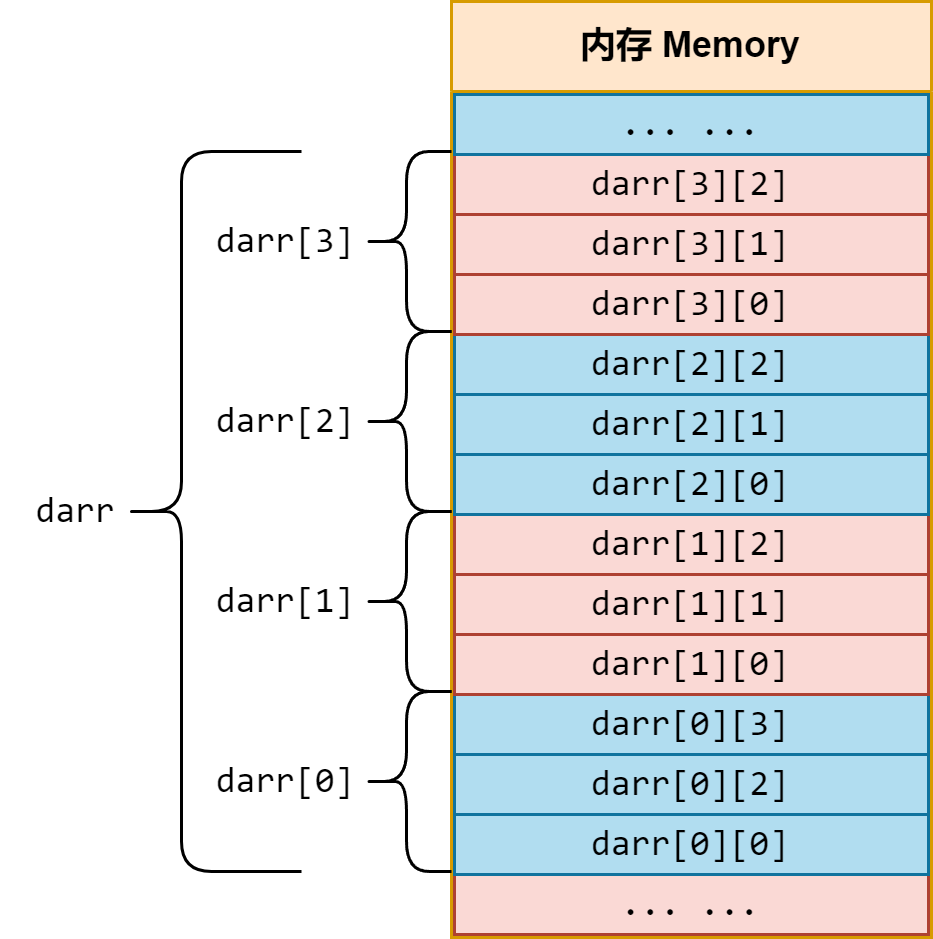
\includegraphics[width=0.6\textwidth]{../images/generalized_parts/05_data_in_the_array_of_array.drawio.png}
    \caption{二维数组在内存中的布局}
    \footnotesize{本图的每个蓝/粉色方框代表一个数据,而非一个字节}
\end{figure}
一些资料会在讲解二维数组时把它画成矩阵的形状,这可能会给读者造成一种误解,即二维数组在内存中是以行列的方式排布的。这是一种偏见。实际情况是,数据在内存中的排布是线性的,比如 \lstinline@darr[0][3]@ 的下一位是 \lstinline@darr[1][0]@,而不是 \lstinline@darr[1][3]@ 或者别的什么。\par
敏锐的读者可能会想,既然 \lstinline@darr[0][3]@ 的下一位就是 \lstinline@darr[1][0]@,那么我们能否通过\linebreak\lstinline@darr[0][4]@ 这样的语法来访问 \lstinline@darr[1][0]@ 呢?这当然是可以的;但是如果我们只用 \lstinline@darr[0][i]@ 来访问 数组数据的话,为什么我们要定义成二维数组呢?直接用一维的不是更方便吗?\par
\subsubsection*{二维数组的常见应用}
接上文,既然二维数组数据在内存中的排布方式与一维数组一样,那么我们之所以会使用二维数组,肯定是因为二维数组在语法上有过人之处。这里我就来介绍一下它的几个常见应用:
\begin{itemize}
    \item 矩阵。设想我们需要存储一个 \lstinline@5*5@ 大小的矩阵。如果用一维数组的话,我们需要用一个大小为 \lstinline@25@ 的矩阵;在表示``第 \lstinline@n@ 行,第 \lstinline@m@ 列''数据的时候,我们需要写成 \lstinline@arr[(n-1)*5+(m-n)]@(别忘记数组下标从 \lstinline@0@ 开始)。但是我们可以用一个大小为 \lstinline@5*5@ 的二维数组直接存储;表示时直接用 \lstinline@darr[n-1][m-1]@ 就行了。这样就很方便吧。
    \item 多个字符串。字符串本身就是一个 \lstinline@char[N]@ 类型的数组。那么当我们需要批量处理字符串时,当然就要用``数组的数组''啦!
    \item 数据统计。有些时候我们需要记录两组数据并作统计分析,例如对``售价''-``利润''数据进行存储。我们当然可以使用两个一维数组来实现这个功能,但是用一个二维数组会在传参时更方便一点!我们可以直接传递一个二维数组,而不是传递两个一维数组。\footnote{需要注意一点,用二维数组的前提是这个二维数组中的所有数据都是同一类型。如果涉及到``名字''-``性别''-``年龄''这样不同数据类型同时存在的情况,我们就需要用结构体,详见第六章。}
\end{itemize}
这里提及到了二维数组参数传递的问题,我们留到待会儿讲指向数组的指针时再讲解。\par
\subsection*{指针数组}
二维数组的表象看上去好像很复杂,其实经过解析之后我们就会发现,那只不过是一种``以数组作为构成元素''的一维数组罢了。指针数组也是这个道理,它是一种``以指针作为构成元素''的一维数组!\par
指针也是一种数据类型,它一经定义,就在内存中有自己的一席之地。假如说有一个场合,需要我们批量定义指针,那么\textbf{指针数组(Array of pointers)}就派上用场了。\par
定义指针数组的基本语法如下:
\begin{lstlisting}
const char *ap1[3] = {"Alice", "Bob", nullptr}; //正常格式
int *ap2[10] {}; //省略的部分将初始化为nullptr
float *ap3[] {nullptr, nullptr, nullptr}; //可以省略指针数组的长度
\end{lstlisting}
初学者很容易把指针数组的定义语法与下文要讲的指向数组的指针搞混,我们在这里还是按照刚才说的原则来解释:``定义的语法''要与``使用的语法''保持一致。\par
\subsubsection*{指针数组是什么?}
这里要提问读者:\lstinline@*ap1[0]@ 是什么?根据C++运算符优先级的知识,我们知道 \lstinline@[]@ 的优先级高于 \lstinline@*@,所以它应该被理解为 \lstinline@*(ap1[0])@。那么 \lstinline@ap1[0]@ 是什么?按照我们的理解,它应该是指针数组的第一个元素——一个指针。那么 \lstinline@*ap1[0]@ 就相当于再对这个指针取内容。而 \lstinline@ap1[0]@ 指向的是字符串字面量 \lstinline@"Alice"@,那么我们不难想见,\lstinline@*ap1[0]@,或者等效于 \lstinline@(ap1[0])[0]@,就是字符 \lstinline@'A'@。\par
我们同样可以用 \lstinline@typeid@ 来检验它们的类型。
\begin{lstlisting}
    cout << typeid(ap1).name() << endl; //输出ap1的类型
    cout << typeid(ap1[0]).name() << endl; //输出ap1[0]的类型
    cout << typeid(*ap1[0]).name() << endl; //输出*ap1[0]的类型
\end{lstlisting}
这段代码的运行结果是\\\noindent\rule{\linewidth}{.2pt}\texttt{
A3\_PKc\\
PKc\\
c
}\\\noindent\rule{\linewidth}{.2pt}
其中的 \lstinline@PKc@ 意为``指向常量 \lstinline@char@ 的指针'',总之是一个指针就对了;而 \lstinline@A3_PKc@ 当然就是一个指针数柤\footnote{其实我们可以分得更细,它是一个``指向常量的指针数组''(Array of pointer to constant),不过初学阶段的读者就不必深究了。}。\par
\subsubsection*{指针数组在内存中是什么样的?}
指针数组在内存中的结构非常简单,它就是一个普通的一维数组而已,只是元素类型换成了指针。指针类型的数据在内存中也有其存储空间,我们稍后再谈。\par
\subsubsection*{指针数组的常见应用}
我们在前面已经看到了指针数组的一个常见应用,那就是存储字符串字面量。我们此前已经提过,字符串字面量不同于其它类型的字面量,它是有地址的!既然它有自己的地址,那么我们没必要再建立一个二维数组,并把这些内容复制到这个二维数组中(既浪费存储空间,又浪费存储所用的时间);而是直接用一批 \lstinline@const char*@ 来指向这些内容就行,什么时候需要就拿出来用。\par
当然这样做的前提是你不需要修改这些字符串字面量的值。如果修改这些值,就可能发生未知错误(这也就是我们使用 \lstinline@const@ 的原因)。\par
指针数组还可以用于动态内存管理。在涉及动态内存分配时,我们可以把一个二级指针通过动态内存分配变为指针数组,然后对其中的每个指针再进行动态内存分配,诸如此类,我们留到下一节再讲。\par
在传递参数时,我们也可能用到指针数组。这和我们用数组类传递参数有着异曲同工之处——如果参数太多,那么用一个数组来传参就要经济得多;如果要传递的指针太多,那么用一个指针数组来存储这些指针,把它作为实参传递给函数,也要经济得多。\par
\subsection*{指向数组的指针}
\textbf{指向数组的指针(Pointer to array,简称数组指针)},对初学者来说更是一个难题。很多初学者搞不清楚什么是指向数组的指针,什么是指针数组,并且经常在定义的时候搞混。这里我们不仅要讲清楚指向数组的指针是什么,还要理清它和指针数组之间是什么关系。\par
定义一个指向数组的指针的基本语法如下:
\begin{lstlisting}
int (*pta1)[5] = {nullptr}; //正常格式,等号可省略
double arr[3] {}; //这只是一个数组
double (*pta2)[3] {&arr}; //3不可省略,并且需要和arr的长度保持一致!
\end{lstlisting}
不要小看定义语句中的 \lstinline@()@,它是指向数组的指针区别于指针数组的关键。\par
\subsubsection*{指向数组的指针是什么?}
顾名思义,这个指针是指向数组的。我们之前遇到的那些指针,它们都是指向数据的。现在我们遇到了指向数组的指针,不用怕,我们把数组也当成一种数据类型就好。(还记得吗,如果我们把一维数组当成一个数据类型的话,二维数组其实就是``一维数组构成的一维数组'')\par
如图5.15所示,现在有一个二维数组 \lstinline@int darr[4][3]@。它的每个元素都是一个长度为3的 \lstinline@int@ 数组(\lstinline@int[3]@),那么我们可以定义一个指向 \lstinline@darr[0]@ 的指针,如下所示:
\begin{lstlisting}
    int (*pta)[3] {&darr[0]};
\end{lstlisting}
在这里我们要解决两个问题。第一,怎么理解它的定义语法?第二,二维数组和指向数组的指针究竟有什么关系?为什么我们可以用 \lstinline@pta@ 指向 \lstinline@darr[0]+0@?\par
首先,让我们来考虑一下使用的语法。\lstinline@(*pta)[0]@ 是什么?这里 \lstinline@(*pta)@ 套了括号,所以应该先算它。鉴于 \lstinline@pta@ 是一个指向数组的指针,那么 \lstinline@(*pta)@ 就是一个数组了。所以 \lstinline@(*pta)[0]@ 就是这个数组的第一个元素,就这么简单。现在读者可以再回看一下指针数组的定义,并比较它们``使用的语法'',大概就可以分清它们的定义语法了吧!\par
我们也可以用 \lstinline@typeid@,一试便知。
\begin{lstlisting}
    cout << typeid(pta).name() << endl;
    cout << typeid(*pta).name() << endl;
    cout << typeid((*pta)[0]).name() << endl;
\end{lstlisting}
这段代码的运行结果是:\\\noindent\rule{\linewidth}{.2pt}\texttt{
PA3\_i\\
A3\_i\\
i
}\\\noindent\rule{\linewidth}{.2pt}
读者可以自行尝试分析之,不难。\par
再来看看二维数组和指向数组的指针间的关系。我们之前说过,\lstinline@T@ 类型数据构成的数组 \lstinline@T[N]@ 可以隐式转换成指向 \lstinline@T@ 类型的指针,即 \lstinline@T*@。对于二维数组也是如此!既然一个二维数组就是一维数组构成的一维数组,那么它就可以转换成指向一维数组的指针!\par
那么读者也可以猜一下,\lstinline@pta+1@ 会指向什么呢?既然指针的加减法讲究的是数据的偏移量而非地址的偏移量,那么我们就应该想到,\lstinline@pta+1@ 应该指向下一个数组,也就是 \lstinline@darr[1]@。同理,\lstinline@pta+2@ 应该指向下一个数组,即 \lstinline@darr[2]@,以此类推。图5.15给出了这种关系,读者可以作为参考。\par
\begin{figure}[htbp]
    \centering
    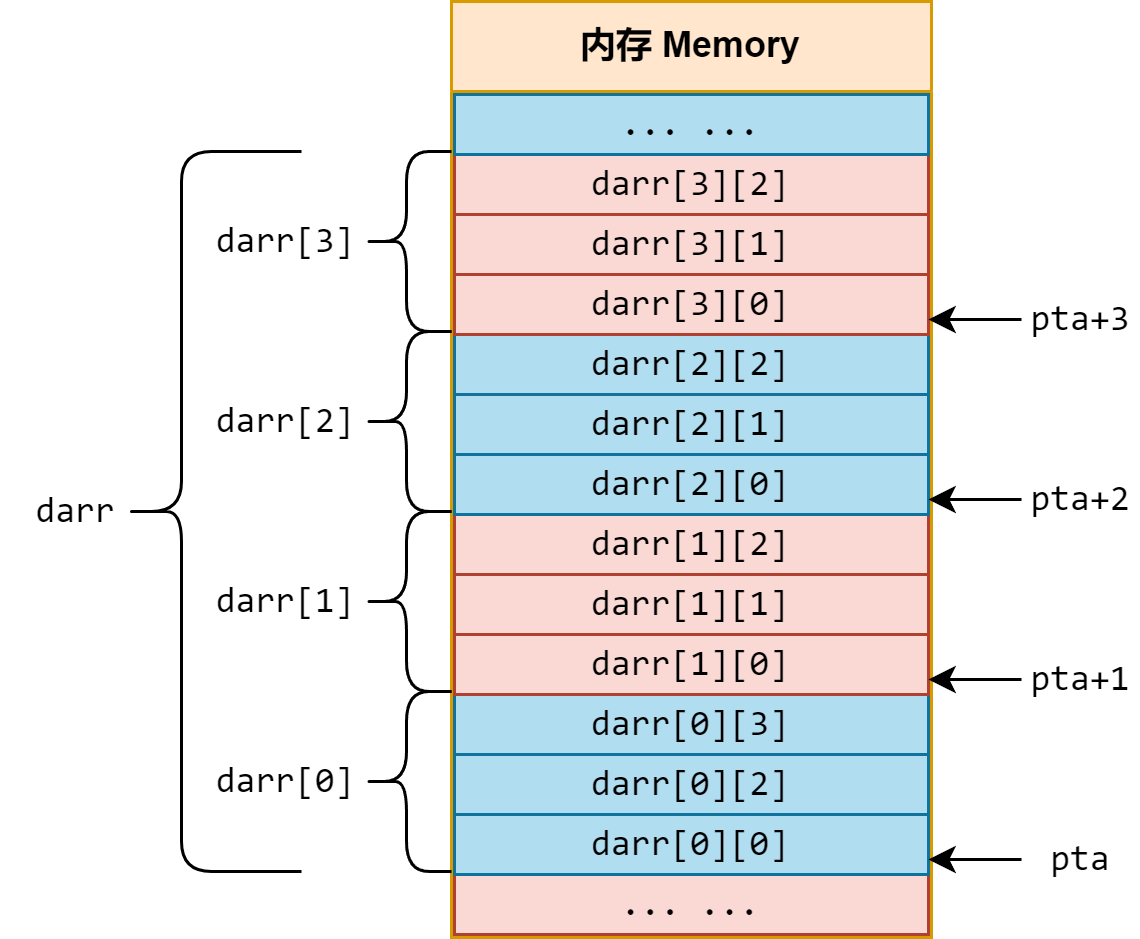
\includegraphics[width=0.75\textwidth]{../images/generalized_parts/05_the_pointer_to_array_and_2d_array.drawio.png}
    \caption{指向数组的指针 \lstinline@pta@ 指向了数组 \lstinline@darr[0]@}
\end{figure}
\subsubsection*{指向数组的指针在内存中是什么样的?}
指向数组的指针只是一个指针。如果你用 \lstinline@sizeof@ 取它的内存占用,会发现它的大小和指向 \lstinline@int@ 的指针相等。实际上,无论指针指向什么,它永远都只是负责存储那个事物的地址而已,所以寥寥几个字节的空间足够!\par
这也就是我们喜欢用指针或引用\footnote{如前文所说,C++中的引用也是通过指针实现的。}传递参数的原因——无论要传递的信息量有多大,一个指针那么大的数据就可以说明一切了!\par
\subsubsection*{指向数组的指针的常见应用}
要说数组指针最常见的应用,那当属二维数组参数传递了。\par
我们说过,所有的数组参数传递在本质上都是指针传递。对于二维数组也是这样。所有的二维数组在进行参数传递时都会被隐式类型转换成指向一维数组的指针,然后传递参数。
\begin{lstlisting}
double MatrixSum(double matrix[][n], int rows);
\end{lstlisting}
这个函数就可以用来求一个矩阵中所有数字的和。\par
一个数组也有它的内存地址。比如说有一个一维数组 \lstinline@arr@,我们可以输出它的地址,也可以直接把它当作指针来输出。
\begin{lstlisting}
    int arr[3];
    cout << arr; //arr会转换成int*型然后输出
    cout << &arr; //直接输出一个int(*)[3],这就是指向数组的指针类型
\end{lstlisting}
它的输出将会是这样的:\\\noindent\rule{\linewidth}{.2pt}\texttt{
0x7ffd12a60744\\
0x7ffd12a60744
}\\\noindent\rule{\linewidth}{.2pt}\par
读者可能会感到奇怪:这两个地址一样啊!\par
没错,这两个地址的值是一样的,但它们的类型完全不同。对于 \lstinline@arr@ 来说,它是 \lstinline@int[3]@ 类型,而在输出的时候会转换成 \lstinline@int*@ 类型。而对数组取地址将会得到 \lstinline@int(*)[3]@ ,这是一个``指向3长度 \lstinline@int@ 数组的指针''类型。我们可以用 \lstinline@typeid@ 或者 \lstinline@is_same@ 来验证它。
\begin{lstlisting}
    cout << is_same<decltype(arr), int[3]>::value << endl; //输出1
    cout << is_same<decltype(&arr), int(*)[3]>::value << endl; //输出1
\end{lstlisting}\par
还记得我曾经说过吗?对于一个需要用多个字节来存储的类型来说,它的地址就是存储区域中第一个字节的地址。\lstinline@arr@ 的第一个字节也正是 \lstinline@arr[0]@ 的第一个字节,地址为 \lstinline@0x7ffd12a60744@,所以自然会输出相同的值,读者不必感到奇怪。如果输出了不一样的值,我们才要感到不对劲呢。\par
那么我们是不是还能想到一种输出字符串字面量地址的新思路?
\begin{lstlisting}
    cout << &"Hello World!"; //将输出地址值
\end{lstlisting}
这里的 \lstinline@&"Hello World!"@ 也是一个指向数组的指针类型,具体地说,是 \lstinline@const char(*)[13]@。
\begin{lstlisting}
    cout << is_same<decltype(&"Hello World!"),const char(*)[13]>::value;
    //输出为1
\end{lstlisting}\par
但是也要提醒读者,这种方法仅适用于字面量;对于指针(哪怕是常量表达式指针)就不如此了。
\begin{lstlisting}
    constexpr static const char *str {"cppHusky"}; //再怎么限制都是不行的啦
    cout << (void*)str << endl;
    cout << &str; //这两个输出结果可是不一样的
\end{lstlisting}
这是因为,当我们计算 \lstinline@&str@ 时,它的返回值是 \lstinline@str@ 自己的地址而不是它指向的事物,是一个二阶指针类型。\par
\subsection*{二阶指针}
我们在前文中说过,一个指针也有它的内存地址。那么我们可以通过取地址运算符来求出它的地址。
\begin{lstlisting}
    int num {3};
    int *p {&num};
    cout << &p << endl << &num;
\end{lstlisting}
这个程序的运行结果是\\\noindent\rule{\linewidth}{.2pt}\texttt{
0x7ffd7e034998\\
0x7ffd7e034994
}\\\noindent\rule{\linewidth}{.2pt}\\
不同于我们在前面看到的例子,这里的 \lstinline@&p@ 和 \lstinline@&num@ 是不同的。\par
它们当然不同啦,又不是同一个数据,也没有包含关系,当然应该存储在不同的单元中。\par
那么我们能否用另一个指针来指向 \lstinline@p@ 呢?这是可以的。我们可以定义一个二阶指针,或者说,指向指针的指针,来实现这个功能。\par
定义一个二阶指针的基本语法如下:
\begin{lstlisting}
    int **pp1 = {&p}; //正常格式,等号可省略
    char **pp2 {}; //省略将默认初始化为nullptr
\end{lstlisting}
这个语句的定义就很容易理解了,不会涉及什么误解。\par
\subsubsection*{二阶指针是什么?}
初学者容易在自己尝试的时候写出 \lstinline@&&num@ 这样的语法,试图一步到位,得到一个二阶指针。这样写是错误的,而且也是没有意义的。这是因为,二阶指针描述的是一个指针的地址。但是 \lstinline@&num@ 只是一个临时的返回值\footnote{更确切地说,右值。我们会在精讲篇中探讨这个问题。},我们不应该在内存中获取到相应的实体,所以对它取地址是没有意义的!\par
但是我们可以对二阶指针两次取内容,这是因为,只要它是一个地址,它就可以取内容。二阶指针存储了某个一阶指针的地址值,我们可以取内容得到一阶指针;而一阶指针又存储了某个数据的地址值,所以我们可以取内容得到对应的数据。总之,我们可以对二阶指针连续取地址。
\begin{lstlisting}
    cout << typeid(pp1).name() << endl;
    cout << typeid(*pp1).name() << endl;
    cout << typeid(**pp1).name() << endl;
\end{lstlisting}
这段代码的运行结果是\\\noindent\rule{\linewidth}{.2pt}\texttt{
PPi\\
Pi\\
i
}\\\noindent\rule{\linewidth}{.2pt}\\
很好理解,我就不多说了。\par
\subsubsection*{二阶指针在内存中是什么样的?}
同上文,它是一个单独的变量,在内存中有它自己的一席之地。我们甚至还可以取二阶指针的地址,并把它存入三阶指针当中!
\begin{lstlisting}
    int ***ppp {&pp1}; //这是一个三阶指针,存储了一个二阶指针的地址
\end{lstlisting}
还有更高阶的指针,不过我们在这里就不多说了。\par
\subsubsection*{二阶指针的常见应用}
我们知道,一个二维数组可以隐式转换成指向数组的指针。而一个指针数组也可以转换成一个二阶指针。其实这点也符合我们的规律,因为它是一个``由指针构成的数组''向``指向指针的指针''的转换。所以如果我们需要向某函数传递一个指针数组,我们就需要用二级指针形参来接收了。\par
这四种类型的转换关系可以用图5.16来描述。注意,二维数组是不能直接转换成二级指针类型的,数组指针也是不能直接转换成指向数组的指针类型的。这方面更详细的讨论,我们放在精讲篇。\par
\begin{figure}[htbp]
    \centering
    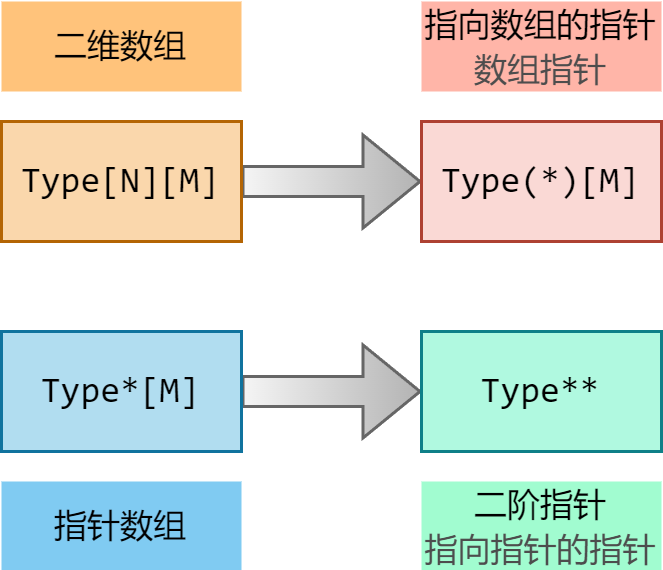
\includegraphics[width=0.5\textwidth]{../images/generalized_parts/05_type_conversions_between_array_and_pointer.drawio.png}
    \caption{四种指针/数组复合类型的类型转换关系}
\end{figure}\par
